\documentclass{beamer}
\usepackage{graphicx}
\usepackage{amsmath}
\usepackage{amsfonts}
\usepackage{amssymb}
\usepackage{listings}
\usepackage{tikz}
\definecolor{mygray}{rgb}{0.92,0.92,0.92}
\usetheme{Montpellier}
\usecolortheme{beaver}

\begin{document}

\section{Group Meeting}
\title{Group Meeting \\ Week 4, Spring 2019}
\author{Brandon Gusto} %
\institute{Dept. of Scientific Computing \\ Florida State University}
\date{\today}
\frame{\titlepage}

\section{Multiresolution Scheme}

\begin{frame}{Hybrid Wavelet/AMR Scheme}
    \begin{columns}
        \begin{column}{0.58\textwidth}
            The goal of this project is to marry the benefits of wavelet analysis with the more developed AMR strategies:
            \begin{itemize}
                \item can wavelet sensors augment LTE for refinement?
                \item can regularity information reduce computational expense on fine grids?
            \end{itemize}
        \end{column}
        \begin{column}{0.44\textwidth}
            \scalebox{0.4}{
                \input{plots/detail_j3.tex}
            }
        \end{column}
    \end{columns}
\end{frame}

\begin{frame}{Harten's MR Scheme}
    The one-dimensional reference system of conservation laws is
    \begin{equation*}
        \mathbf{U}_{t} + \mathbf{F}(\mathbf{U})_{x} = 0,
    \end{equation*}
    where $\mathbf{U} = (\rho,\rho u,E)$ is a vector of conserved quantities.
    In semi-discrete form,
    \begin{equation*}
        \frac{\partial \mathbf{U}_{i}}{\partial t} = -\frac{1}{h} \left( \mathbf{F}_{i+\frac{1}{2}}
            - \mathbf{F}_{i-\frac{1}{2}} \right) = \mathbf{R}_{i}
    \end{equation*}
    where the $i$ denotes spatial index, and $\mathbf{R}$ is residual.
\end{frame}

\begin{frame}{Harten's MR Scheme}
    Define multiple, nested grids
    \begin{equation*}
        \mathbf{G}^{l} = \left\{ x^{l}_{i+\frac{1}{2}} \right\}_{i=0}^{N_{l}} =
            \left\{ x^{l+1}_{i+\frac{1}{2}} \right\}_{i=0,\text{i even}}^{N^{l+1}}.
    \end{equation*}
    Coarsening of a cell done via
    \begin{equation*}
        \mathbf{U}^{l}_{i} = \frac{1}{2} \left( \mathbf{U}^{l+1}_{2i} + \mathbf{U}^{l+1}_{2i+1} \right)
    \end{equation*}
    and the prediction from coarse to fine is
    \begin{equation*}
        \mathbf{\hat{U}}^{l+1}_{2i+1} = \sum_{j=1-s}^{s-1} \gamma_{l} \mathbf{U}^{l}_{i+l}
    \end{equation*}
\end{frame}

\begin{frame}{Harten's MR Scheme}
    The regularity information is assessed by computing detail coefficients as
    \begin{equation*}
        \mathbf{d}^{l}_{i} = \mathbf{U}^{l+1}_{2i+1} - \mathbf{\hat{U}}^{l+1}_{2i+1}.
    \end{equation*}
    A mask $\left\{ \mathbf{m} \right\}_{i}^{N^{l}}$ is created for significant cells. The fluxes are initially computed on
    coarsest level, then via
    \begin{align*}
        & \mathbf{F}^{l+1}_{2i-\frac{1}{2}} = \mathbf{F}^{l}_{i-\frac{1}{2}} \\
        & \text{if} \text{ } m_{i}^{l} == true, \text{then} \text{ } \mathbf{F}^{l+1}_{2i+\frac{1}{2}} = \mathbf{F}(\mathbf{U}) \\
        & \text{else} \text{ } \text{interpolate...}
    \end{align*}
\end{frame}

\begin{frame}{Multiresolution Representation}
% cell average drawing
\begin{figure}
    \centering
    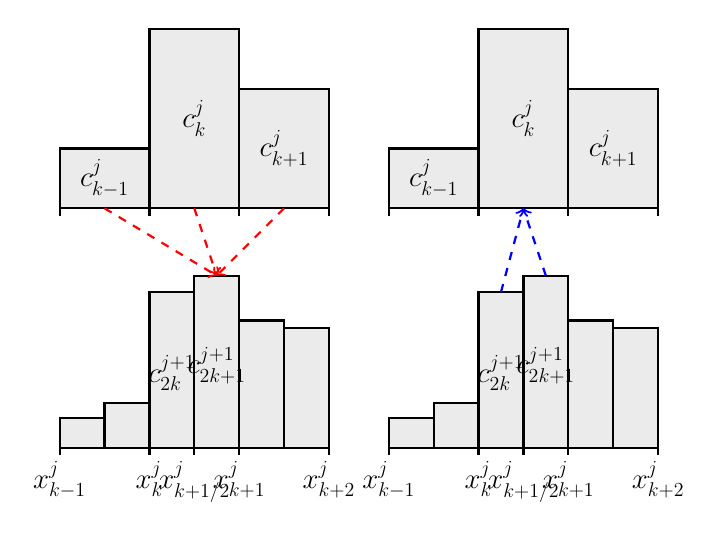
\begin{tikzpicture}[thick,scale=0.38, every node/.style={scale=0.6}]

        % variables
        \def\x{-8.0}
        \def\y{0.0}
        \def\yl{-8.0}

        % draw coarse level rectangles
        \draw [fill=mygray] (\x,0) rectangle (\x+3,2);
        \draw [fill=mygray] (\x+3,0) rectangle (\x+6,6);
        \draw [fill=mygray] (\x+6,0) rectangle (\x+9,4);

        % coarse level symbols
        \node at (\x+1.5,1) {\LARGE $c^{j}_{k-1}$};
        \node at (\x+4.5,3) {\LARGE $c^{j}_{k}$};
        \node at (\x+7.5,2) {\LARGE $c^{j}_{k+1}$};

        % coarse level axis
        \draw (\x,0) -- (\x,-0.25);
        \draw (\x+3,0) -- (\x+3,-0.25);
        \draw (\x+6,0) -- (\x+6,-0.25);
        \draw (\x+9,0) -- (\x+9,-0.25);

        % fine level rectangles
        \draw [fill=mygray] (\x,\yl) rectangle (\x+1.5,\yl+1);
        \draw [fill=mygray] (\x+1.5,\yl) rectangle (\x+3,\yl+1.5);
        \draw [fill=mygray] (\x+3,\yl) rectangle (\x+4.5,\yl+5.2);
        \draw [fill=mygray] (\x+4.5,\yl) rectangle (\x+6,\yl+5.75);
        \draw [fill=mygray] (\x+6,\yl) rectangle (\x+7.5,\yl+4.25);
        \draw [fill=mygray] (\x+7.5,\yl) rectangle (\x+9,\yl+4.0);

        % fine level symbols
        \node at (\x+3.75,\yl+2.5) {\LARGE $c^{j+1}_{2k}$};
        \node at (\x+5.25,\yl+2.75) {\LARGE $c^{j+1}_{2k+1}$};

        % fine level axis
	    \draw (\x,\yl) -- (\x,\yl-0.25);
        \draw (\x+3,\yl) -- (\x+3,\yl-0.25);
        \draw (\x+4.5,\yl) -- (\x+4.5,\yl-0.25);
        \draw (\x+6,\yl) -- (\x+6,\yl-0.25);
	    \draw (\x+9,\yl) -- (\x+9,\yl-0.25);

        % arrows
        \draw[red,dashed,->] (\x+1.5,\y) -- (\x+5.25,\y-2.25);
        \draw[red,dashed,->] (\x+4.5,\y) -- (\x+5.25,\y-2.25);
        \draw[red,dashed,->] (\x+7.5,\y) -- (\x+5.25,\y-2.25);

        % tick text
        \node[below] at (\x,\yl-0.25) {\LARGE $x^{j}_{k-1}$};
        \node[below] at (\x+3,\yl-0.25) {\LARGE $x^{j}_{k}$};
        \node[below] at (\x+4.5,\yl-0.25) {\LARGE $x^{j}_{k+1/2}$};
        \node[below] at (\x+6,\yl-0.25) {\LARGE $x^{j}_{k+1}$};
        \node[below] at (\x+9,\yl-0.25) {\LARGE $x^{j}_{k+2}$};

        %----

        % variables
        \def\x{3.0}
        \def\y{0.0}
        \def\yl{-8.0}

        % draw coarse level rectangles
        \draw [fill=mygray] (\x,0) rectangle (\x+3,2);
        \draw [fill=mygray] (\x+3,0) rectangle (\x+6,6);
        \draw [fill=mygray] (\x+6,0) rectangle (\x+9,4);

        % coarse level symbols
        \node at (\x+1.5,1) {\LARGE $c^{j}_{k-1}$};
        \node at (\x+4.5,3) {\LARGE $c^{j}_{k}$};
        \node at (\x+7.5,2) {\LARGE $c^{j}_{k+1}$};

        % coarse level axis
        \draw (\x,0) -- (\x,-0.25);
        \draw (\x+3,0) -- (\x+3,-0.25);
        \draw (\x+6,0) -- (\x+6,-0.25);
        \draw (\x+9,0) -- (\x+9,-0.25);

        % fine level rectangles
        \draw [fill=mygray] (\x,\yl) rectangle (\x+1.5,\yl+1);
        \draw [fill=mygray] (\x+1.5,\yl) rectangle (\x+3,\yl+1.5);
        \draw [fill=mygray] (\x+3,\yl) rectangle (\x+4.5,\yl+5.2);
        \draw [fill=mygray] (\x+4.5,\yl) rectangle (\x+6,\yl+5.75);
        \draw [fill=mygray] (\x+6,\yl) rectangle (\x+7.5,\yl+4.25);
        \draw [fill=mygray] (\x+7.5,\yl) rectangle (\x+9,\yl+4.0);

        % fine level symbols
        \node at (\x+3.75,\yl+2.5) {\LARGE $c^{j+1}_{2k}$};
        \node at (\x+5.25,\yl+2.75) {\LARGE $c^{j+1}_{2k+1}$};

        % fine level axis
	    \draw (\x,\yl) -- (\x,\yl-0.25);
        \draw (\x+3,\yl) -- (\x+3,\yl-0.25);
        \draw (\x+4.5,\yl) -- (\x+4.5,\yl-0.25);
        \draw (\x+6,\yl) -- (\x+6,\yl-0.25);
	    \draw (\x+9,\yl) -- (\x+9,\yl-0.25);

        % arrows
        \draw[blue,dashed,->] (\x+5.25,\y-2.25) -- (\x+4.5,\y);
        \draw[blue,dashed,->] (\x+3.75,\y-2.8) -- (\x+4.5,\y);

        % tick text
        \node[below] at (\x,\yl-0.25) {\LARGE $x^{j}_{k-1}$};
        \node[below] at (\x+3,\yl-0.25) {\LARGE $x^{j}_{k}$};
        \node[below] at (\x+4.5,\yl-0.25) {\LARGE $x^{j}_{k+1/2}$};
        \node[below] at (\x+6,\yl-0.25) {\LARGE $x^{j}_{k+1}$};
        \node[below] at (\x+9,\yl-0.25) {\LARGE $x^{j}_{k+2}$};


    \end{tikzpicture}
    \caption{Left: quadratic prediction from coarse-scale $j$
        to fine-scale $j+1$, given cell-averages $\mathbf{c}^{j}$.
        Right: Fine-scale cell averages are coarsened.}

\end{figure}
\end{frame}

\section{Multiresolution Code}

\begin{frame}{Multiresolution Code - Examples}
	\begin{figure}
		\center
		\includegraphics[scale=0.5]{plots/spike-med.png}
		\caption{Better approximation (smaller threshold value).}
	\end{figure}
\end{frame}

\section{Multiresolution Finite Volume Scheme}

\begin{frame}{Multiresolution Scheme on AMR Patches}
	\begin{figure}
		\center
		\includegraphics[scale=0.5]{plots/patch-efficiency.png}
		\caption{Increasing patch 'efficiency.'}
	\end{figure}
\end{frame}

\begin{frame}{Multiresolution Scheme on AMR Patches}
      The steps of the scheme for one patch are
      \begin{enumerate}
        \item take given (finest level) data on patch, and coarsen it to desired coarsest level $L$
        \item compute the forward wavelet transform to obtain $\left\{ \mathbf{d}^{l}\right\}_{l=L}^{l=1}$
        \item on coarsest level $L$, compute the residuals $\left\{ R_{j}^{L} \right\}_{j=0}^{N_{L}}$
        \item loop through one finer level at a time, and according to detail coefficients,
              either interpolate or calculate remaining fluxes
      \end{enumerate}
\end{frame}

\begin{frame}{Multiresolution Scheme on AMR Patches}
  The original (fine) data is coarsened by
      \begin{equation*}
        w_{j}^{l} = \frac{1}{2} \left( w_{2j}^{l-1} + w_{2j+1}^{l-1} \right)
      \end{equation*}
      Then the residual $R_{j}^{l}$ may be interpolated in smooth regions as
      \begin{align*}
        R^{l-1}_{2j+1} & = R^{l}_{j} - \frac{1}{8} \left( R^{l}_{j-1} - R^{l}_{j+1} \right) \\
        R^{l-1}_{2j} & = 2 R^{l}_{j} - R^{l-1}_{2j+1}
      \end{align*}
\end{frame}

\begin{frame}[fragile]{Progress in FLASH Implementation}
  \begin{itemize}
    \setlength\itemsep{1em}
    \item created a new folder \texttt{source/flashUtilities/Wavelet/}
    \item writing a program \texttt{Wavelet\_computeTransform.F90} which will be run 
          in \texttt{Grid\_computeUserVars.F90}
  \end{itemize}
  \begin{verbatim}
    function imap( l, i, j, k, nx, ny, nz ) result(x)
      integer, intent(in) :: nx(:), ny(:), nz(:)
      integer, intent(in) :: l, i, j, k
      integer             :: x

      ! compute the map
      x = l + nx * ( i + ny * ( j + nz * k ) )

    end function imap
  \end{verbatim}
\end{frame}


\end{document}
